 %***************************************************************************%
 % Thesis work                                                               %
 %                                                                           %
 %                                                                           %
 %                        B A C H E L O R   T H E S I S                      %
 %                                                                           %
 %                                                                           %
 %  Title:                                                                   %
 %                                                                           %
 %  Author:                                                                  %
 %                                                                           %
 %  Supervisor:                                                              %
 %                                                                           %
 %  Date:                                                                    %
 %                                                                           %
 %***************************************************************************%

 %   Template - Institute of Control Systems, TUHH
 %
 %   G. Lichtenberg
 %
 %   Updates:
 %   GL: 31.07.2007
 %   AP: 29.08.2007
 %
 %   Version 2.2

 %##########################################
 %     R E A D      M E     F I R S T  !
 %##########################################
 % Possible compilation processes:
 % LaTeX -> DVI -> PS -> PDF   
 % LaTeX -> pdfTeX -> PDF
 %##########################################

 %%################ Document  settings ###################
%%%%%%%%%%%%%%%% Document settings %%%%%%%%%%%%%%%%%%%%
\NeedsTeXFormat{LaTeX2e}

\RequirePackage{ifpdf}	%% detection of pdfTeX or DVI
\ifpdf
	\documentclass[a4paper,12pt]{article}
\else
	\documentclass[a4paper,12pt,dvipdfm]{article}
\fi

\usepackage{graphicx}                %% special graphics
\usepackage{color}                   %% allow colour
\usepackage{latexsym}                %% symbols package
\usepackage{amsmath}                 %% special mathematical functions
\usepackage{theorem}
\usepackage{amsfonts}
%\usepackage{multirow}                %% multirow tables



 %%############### Choose LANGUAGE
 %%% English
%	\usepackage[english]{babel}
%	\selectlanguage{english}

 %%% German
	\usepackage[english, german]{babel}
	\selectlanguage{german}
   % %% In some cases you might need that
   % \usepackage{german}
	\usepackage[latin1]{inputenc}


 %%############### Functions and Hyphenation rules
\newcommand{\bbma} {\begin{bmatrix} }
\newcommand{\ebma} {\end{bmatrix}}
\newcommand{\real} {\mathbb{R}}
\newcommand{\vs}[1]{\vspace{#1mm}}


\hyphenation{Trenn-ungs-re-geln meh-re-re}


 %%############### Enumeration of figures and equations
\numberwithin{figure}{section}
\numberwithin{equation}{section}
\newtheorem{definition}{Definition}[section]
\newtheorem{theorem}{Theorem}[section]


 %%############### Figures
\graphicspath{{figures/}} 				% Folder with the figures

\ifpdf % pdfTeX
	\DeclareGraphicsExtensions{.pdf,.png,.jpg,.gif,.pdftex}
	\DeclareGraphicsRule{.pdftex}{pdf}{*}{}	% for xfig exported files
	\newcommand{\xfig}[2]{\scalebox{#1}{\input{"figures/#2.pdftex_t"}}} % XFIG

\else % DVI
	\DeclareGraphicsExtensions{.eps,.pstex}
	\DeclareGraphicsRule{.pstex}{eps}{*}{}		% for xfig exported files
	\newcommand{\xfig}[2]{\scalebox{#1}{\input{"figures/#2.pstex_t"}}} % XFIG
	%\usepackage{psfrag}		% might be useful
\fi

 % Other figures (e.g., MATLAB  EPS or PDF figures)
\newcommand{\afig}[2]{\includegraphics[scale=#1]{#2}}

 % figures defined in TeX files
\newcommand{\tfig}[2]{\scalebox{#1}{\input{"#2.tex"}}}







 %%############### Hyper References Settings
%\ifpdf % pdfTeX
%\else
\usepackage[
%a4paper=true;
%letterpaper=false;
hypertexnames = false,             % hyperlinks
bookmarks=true,
bookmarksnumbered=true,%
linkbordercolor={0 1 1},%        % cyan
urlbordercolor={0 0 1},%         % magenta
plainpages=false,                % false - to fix the hyperpage links for index
pdfsubject={Control Systems}]%
{hyperref}
%\fi





 %%############### Page Size Settings
%%% WAIT - before changing the settings make a back-up copy!!!
%%% For more information about the meaning of the settings check
%%% "The not so short introduction to LaTeX", page 125

\setlength{\hoffset}{-1in}%               % To eliminate the standard offset
\setlength{\voffset}{-1in}%
\setlength{\evensidemargin}{23mm}%
\setlength{\oddsidemargin}{35mm}%
\setlength{\topmargin}{10mm}%
\setlength{\headheight}{30pt}%

\setlength{\headsep}{10mm}%
\setlength{\textheight}{230mm}%
\setlength{\textwidth}{160mm}%
\setlength{\marginparsep}{0mm}%
\setlength{\marginparwidth}{10mm}%
\setlength{\footskip}{10mm}%

\renewcommand{\textfraction}{0}%
\renewcommand{\topfraction}{0.9}%
\renewcommand{\bottomfraction}{0.9}%
\renewcommand{\floatpagefraction}{1.5}

\widowpenalty=10000      % penalty for creating widow line at top of page




 %%############### Paragraph settings

\setlength{\parindent}{0pt}%      % Paragraphs are not indent
\setlength{\parskip}{5pt}%        % space between paragraphs

\setlength{\labelwidth}{0.5cm}%
\setlength{\labelsep}{0.5cm}%

\renewcommand{\baselinestretch}{1.0}




 %%############### % Numbered items
%\setcounter{secnumdepth}{2}            % Number until 3th depth X.Y.Z
%
%\numberwithin{figure}  {section}       % Numbering of for the figures
%\numberwithin{equation}{section}
%
%\newtheorem{definition} {Definition}[section]
%\newtheorem{theorem}    {Theorem}   [section]




 %%###############  Page Style settings
%\usepackage{fancyhdr}                %% extended page layout formating

%\pagestyle{fancy}
%
%\renewcommand{\chaptermark}[1]{\markboth{\thechapter. \MakeUppercase{#1}}{}}
%\renewcommand{\chaptermark}[1]{\markboth{\MakeUppercase{#1}}{}}
%\fancyhf{}%
%\renewcommand{\headrulewidth}{0.4pt}
%\renewcommand{\footrulewidth}{0.0pt}
%
% %% Single sinded
%    \fancyhead[R]{\thepage}%%
%    \fancyhead[L]{\rightmark}%%
% \fancypagestyle{plain}{%
%    \fancyhf{} % get rid of headers
%    \renewcommand{\headrulewidth}{0pt}% get rid of the lines
%    \renewcommand{\footrulewidth}{0pt}% get rid of the lines
%}%
%\makeatletter
%\def\cleardoublepage{\clearpage\if@twoside \ifodd\c@page%
%\else \thispagestyle{empty} \hbox{} \newpage%    
%\fi\fi}%
%\makeatother




 %%#######################################################
 %%################## Document Data ######################
 % Titel der Arbeit
\title{\vspace{2cm} Thermisch-hydraulische Modellierung der Ringleitung-W�rmeversorgungsanlage eines
Industriebetriebs \vspace{3cm}}

% Autoren
\author{Kathrin Weihe \vspace{2cm} \\
 %  Die zutreffende Zeile auskommentieren ...
Betreuer: \\  Prof. Dr.-Ing. Gerwald Lichtenberg \\ M. Sc. Kai Kruppa  \\
  \vspace{2cm} }

\date{\today}


 %%%%%%%%% Include only the sections you work with for faster compilation
%\includeonly{}


 %%##############################  CONTENTS ###################################
\begin{document}

 %% Title page
\thispagestyle{empty}
\maketitle
\cleardoublepage


 %% Erkl�rung der Eigenst�ndigkeit  		%% Declaration
\vspace{3cm}

 %% English
%Hereby I declare that I produced the present work myself only with the help of the indicated aids and sources.

 %% Deutsch
Hiermit erkl�re ich, die vorliegende Arbeit selbstst�ndig durchgef�hrt und keine weiteren Hilfsmittel und Quellen als die angegebenen genutzt zu haben.

\vspace{3cm}

Hamburg, \today  \hfill  Kathrin Weihe


 % R�cksetzen des Seitenz�hlers
\cleardoublepage
%\setcounter{page}{1}

 %% Inhaltsverzeichnis							%% Table of Contents 
\tableofcontents
\cleardoublepage


 %% Sections --------------------------------------------
\section*{Formelzeichen}

\begin{acronym}[ANOVA]
\acro{a}[$A$] Systemmatrix
\acro{b}[$B$] Eingangsmatrix
\acro{c}[$C$] Ausgangsmatrix
\acro{cw}[$c_w$]{spezifische W�rmekapazit�t des Wassers}
\acro{d}[$D$] Durchgriffsmatrix
\acro{e}[$e(k)$]{St�rgr��envektor zum Zeitpunkt $k \cdot T_a$}
\acro{k}[$K$] St�rgr��enmatrix
\acro{kk}[$k \in \mathbb{Z}$]{Abtastschritt}
\acro{m}[$m$]{Masse}
\acro{dotm}[$\dot{m}$]{Massenstrom}
\acro{p}[$P$] Parametermatrix
\acro{qw}[$Q$]{W�rmeenergie}
\acro{ql}[$\dot{Q}$]{W�rmeleistung}
\acro{rho}[$\rho$]{Dichte}
\acro{T}[$T$]{Temperatur}
\acro{Ta}[$T_a$]{Abtastzeit}
\acro{t}[$t$]{Zeit}
\acro{inp}[$u(k)$]{Eingangsgr��e zum Zeitpunkt $k \cdot T_a$}
\acro{V}[$V$]{Volumen}
\acro{dotV}[$\dot{V}$]{Volumenstrom}
\acro{inp}[$x(k)$]{Zustandsvektor zum Zeitpunkt $k \cdot T_a$}
\acro{oup}[$y(k)$]{Ausgangsgr��en zum Zeitpunkt $k \cdot T_a$}
\end{acronym}

\section*{Indizes und Abk�rzungen}
\begin{acronym}[ANOVA]
\acro{4sid}[4SID]{Subspace-based State-Space System Identification}
\acro{hz1}[HZ1]{Heizzentrale 1}
\acro{hz2}[HZ2]{Heizzentrale 2}
\acro{nrmse}[NRMSE]{Normalized Root Mean Square Error}
\acro{q}[q]{W�rmeleistung}
\acro{rue}[R]{R�cklauf}
\acro{vor}[V]{Vorlauf}
\end{acronym}		% Einleitung

\section{Das Schreiben mit LaTeX}\label{a:latex}

\subsection{Das Besondere an LaTeX}

In diesem Kapitel werden Sie einige n�tzliche Hinweise zur
Erstellung von Studien- und Diplomarbeiten mit LaTeX erhalten.
Wichtig zu wissen ist, dass LaTeX kein WYSIWYG (what you see is
what you get) Programm ist wie andere Texteditoren wie z.B.
Microsoft Word. Es ist vielmehr eine Art Programmiersprache, mit
der Sie den logischen Zusammenhang Ihres Textes durch geeignete
Befehle zun�chst beschreiben. Dieser ''Quellcode'' ist die sog.\
LaTeX-Datei.

Es gibt wie bei Programmen eine compilierbare Datei f�r das
Hauptprogramm und u.U.\ weitere Dateien f�r Unterprogramme, die
eingebunden werden (sinnvollerweise sind das hier die Kapitel).
Der Compiler erzeugt aus dem Quellcode entweder eine sog.\
Dvi-Datei (f�r ''device independent'') (LaTeX) oder direkt eine
Pdf-Datei (PdfLaTeX). Aus der Dvi-Datei k�nnen Sie mit dem
Programm dvi2ps dann eine Postscript-Datei erstellen, die dann auf
geeigneten Druckern ausgedruckt werden kann.

Dies gibt Ihnen z.B.\ auch die M�glichkeit im Quellcode Kommentare
einzuf�gen, die im endg�ltigen Text nicht sichtbar sind. Es kommt
dabei auch nicht auf die Zeilenumbr�che im Quellcode an, da diese
erst durch den Compilierungsvorgang erzeugt werden. Das Layout der
fertigen Arbeit k�nnen Sie getrost am letzten Tag Ihrer Arbeit
machen; wenn alle logischen Verkn�pfungen und der Text als solcher
sowie die Bilder stimmig sind, dauert das ca.\ einen Tag. Bedenken
Sie, dass auch das Ausdrucken, insbesondere bei farbigen Seiten
Zeit in Anspruch nimmt!

Die Vorteile von LaTeX werden insbesondere bei Umstellungen des
Textes und beim Formelsatz deutlich. Durch die logische
Referenzierung stimmen die Referenzen immer, die Druckqualit�t von
Formeln wird von anderen Programmen nicht erreicht. Die
Einfachheit des Zitierens ist gerade f�r einen Anf�nger sehr
hilfreich.

Der folgende Text als solcher ist nicht sonderlich sinnvoll, wenn
Sie aber gleichzeitig die Datei mit dem Quellcode lesen, kann man
sehr gut verstehen, wie verschiedene Elemente erzeugt werden. Sie
sollten dann diese Datei auch selbst compilieren und das Ergebnis
vergleichen. Wenn es nicht identisch ist, ist u.U.\ die
LaTeX-Konfiguration nicht korrekt und muss dann korrigiert werden.

\subsection{Normaler Text}

Normalen Text zu schreiben ist ganz einfach. Man nutzt einen
beliebigen Editor und schreibt einfach den Text, ohne auf die
Formatierung, Zeilenumbr�che etc. zu achten. Will man einen neuen
Abschnitt beginnen, so l�sst man einfach eine oder mehrere
Leerzeilen...

Hier sind wir nun im neuen Abschnitt. Die Schriftgr��e wird
�brigens im Kopfteil des Hauptdokumentes definiert. Man kann
Hervorhebungen durch andere Schriftarten machen. Normalerweise
werden neu definierte Begriffe in \textit{italic}, wichtige
Aussagen in \textbf{bold} und Programmzeilen mit \verb"\verb"
gesetzt.

\subsubsection{Gliederungsebenen}

Man kann feinere Unterteilungen der Abschnitte durch den Befehl
''subsubsection'' erreichen. Diese Ebene sollte die unterste Ihrer
Arbeit sein.

\subsubsection*{Gleiche Ebene, aber nicht numeriert}

Sehen Sie in den Quellcode, um zu wissen, wie das erreicht wird!

\subsection{Besondere Objekte}


\subsubsection{Bilder}\label{b:picturesubsection}

Bild \ref{f:picfirstfigure} zeigt ein Blockschaltbild.

\begin{figure}[ht]		% h - here, t - top, b - bottom, p - page, ! - try hard
  \centering
  \afig{1}{example}			% {scaling}{Figure from MATLAB, picture, etc.}
  \caption{Das erste Bild}
  \label{f:picfirstfigure}
\end{figure}

Wenn das Datei durch DVI kompiliert sind (latex $\rightarrow$ dvi $\rightarrow$ pdf, oder latex $\rightarrow$ dvi $\rightarrow$ ps $\rightarrow$ pdf) kann Bild \ref{f:picfirstfigure} PS oder EPS sein. Wenn aber, man kompiliert direkt mit pdfTeX (latex $\rightarrow$ pdf), die Figuren m�ssen JPEG, PDF, PNG, usw. sein -- kein PS oder EPS.


Bild \ref{f:xfigfigure} ist ein Beispiel f�r Diagramm, das mit XFig erzeugt ist. 

\begin{figure}[ht]
  \centering
  \xfig{1}{carts}			% {scaling}{XFig figure}
  \caption{Das zweite Bild}
  \label{f:xfigfigure}
\end{figure}







\subsubsection{Formeln}

Formeln wie diese
\begin{eqnarray}
\ddot{\phi}_1
    &=&
    \frac{M_1+l_1 \sin \phi_2
    (m_2 l_{s2} + m_3 l_{s3})
    (\dot{\phi}_2^2+2 \dot{\phi}_1\dot{\phi}_2 )
    -f_1 \dot{\phi}_1}
    {\theta_1+\theta_2+\theta_3+2l_1 (m_1 l_{s2}+m_3 l_{s3} \cos \phi_2)+
    m_3 (l_1^2+l_2^2)+m_l l_1^2}  \,,  \label{e:eqnfirst} \\
\ddot{\phi}_2
    &=&
    \frac{M_2 + l_1 \sin \phi_2 (m_2 l_{s2} + m_3 l_{s3})
    \dot{\phi}_1^2 +2 - \phi_2 \dot{\phi}_2}
    {\theta_1+\theta_2+\theta_3} \, \label{e:eqnsecond}
\end{eqnarray}
k�nnen in sch�nem Satz ausgedruckt werden. Bitte beachten Sie,
dass auch Formeln zu den S�tzen geh�ren und ebenso Satzzeichen
enthalten k�nnen!


\subsubsection{Symbole}

Symbole wie $\Omega$ k�nnen auch einfach in den Fliesstext mit
aufgenommen werden. S�tze fangen {\bf nie} mit einem Symbol an!


\subsubsection{Zitate}

Zitate werden einfach mit Komma an den Satz angeh�ngt,
\cite{Lu96}. Nachdem man das Programm BiBTeX aufgerufen hat, wird
das Literaturverzeichnis automatisch erstellt. Die Auswahl eines
Zitierstiles erfolgt in der Haupt-Datei.


\subsubsection{Inhaltsverzeichnis}

Das Inhaltsverzeichnis wird automatisch durch LaTeX erstellt. Dazu
schreibt das Programm bei jedem Compilierungslauf  sog.\
aux-Dateien (auxiliary), die alle f�r das Inhaltsverzeichnis
wichtigen Elemente enthalten. Diese Dateien werden dann beim
n�chsten Compilieren mit eingebunden. Wenn


\subsubsection{Referenzen}\label{b:subsecrefer}

Man kann auf Bilder wie das Bild \ref{f:picfirstfigure}, Gleichungen
(\ref{e:eqnsecond}), oder ganze Abschnitte \ref{b:picturesubsection}
verweisen. Sehen Sie, wie das geht? Hierin liegt die eigentliche
St�rke des Programms!


\section{Grundlagen}
Das folgende Kapitel fasst die theoretischen Grundlagen der physikalischen, mathematischen und systemtheoretischen Konzepte zusammen, die in dieser Arbeit Anwendung gefunden haben. Sie sollen dem Leser als Nachschlagewerk dienen und zum Verst�ndnis des in dieser Arbeit gew�hlten Modellierungsansatzes beitragen. Zun�chst werden die thermodynamischen Grundlagen von Heizkreisen erl�utert, anschlie�end folgt ein �berblick �ber das Konzept der Modellbildung und verschiedenen Modellierungstypen. Der letzte Abschnitt des Kapitels befasst sich mit Parameteridentifikation und beschreibt zwei verwendete Ans�tze.

\subsection{Thermodynamik von Heizkreisen}
Heizungsanlagen werden in Geb�uden installiert, um Raumw�rme und Warmwasser bereitzustellen. Die am h�ufigsten anzufindende Art der Heizungsanlage ist dabei die Warmwasserheizung. Hierbei wird Warmwasser durch W�rmeerzeuger bereitgestellt und �ber Umw�lzpumpen durch Heizungsrohre zu Heizk�rpern oder Heizfl�chen transportiert. Besteht ein Temperaturunterschied zwischen der Umgebungstemperatur und der Temperatur des Heizk�rpers, wird unter Abk�hlung des Warmwassers W�rmeenergie 
\begin{equation}
\Delta Q = c_w \cdot m \cdot \Delta T
\label{eq:waermeenergie}
\end{equation}
an die Umgebung abgegeben, wobei $c_w$ der spezifischen W�rmekapazit�t von Wasser, $m$ der Masse und $\Delta T$ der Temperatur�nderung des Wassers entspricht. Wird statt der W�rmeenergie $Q$ die W�rmeleistung $\dot{Q}$ betrachtet, l�sst sich \eqref{eq:waermeenergie} umformen zu
\begin{equation}
\dot{Q} = c_{w} \cdot \dot{m} \cdot \Delta T = c_{w} \cdot \rho \cdot \dot{V} \cdot \Delta T ,
\label{eq:waermemenge}
\end{equation}
mit dem Massenstrom $\dot{m}$, der Dichte von Wasser $\rho$ und dem Volumenstrom $\dot{V}$ . Das auf diese Weise im sogenannten Verbraucher abgek�hlte Wasser wird erneut dem W�rmeerzeuger zugef�hrt, wo das Heizungswasser W�rme aufnimmt und der Heizkreislauf von neuem beginnt,\cite{TBHK90}.

\subsubsection{Erzeuger}
Als W�rmeerzeuger werden in der Regel Heizkessel verwendet, die die chemisch gebundene Energie eines Brennstoffs wie �l, Kohle oder Gas durch Verbrennung in thermische Energie umwandeln. �ber W�rmetauscher wird die thermische Energie an das Heizungswasser �bertragen. Die Temperatur des so erw�rmten Heizwassers wird Vorlauftemperatur genannt. Die Heizleistung eines W�rmeerzeugers kann dabei durch Vorgabe einer Sollgr��e geregelt werden, zum Beispiel durch Vorgabe einer Soll-Vorlauftemperatur, \cite{Her14}. 
\subsubsection{Verbraucher}
Heizk�rper oder Heizfl�chen werden in der Heizungstechnik auch als Verbraucher bezeichnet. Sie entziehen dem Heizkreis W�rme, da durch sie eine W�rme�bertragung durch Konvektion und W�rmestrahlung an den sie umgebenden Raum stattfindet. Tritt Wasser mit einer Vorlauftemperatur $T_V$ in einen Heizk�rper ein, k�hlt sich das Wasser nach \eqref{eq:waermeenergie} ab und tritt mit einer Temperatur $T_R$ < $T_V$ aus dem Heizk�rper wieder aus. Die Temperatur $T_R$ wird auch R�cklauftemperatur genannt.

\subsection{Modellbildung}
Ziel der Modellbildung ist es, ein Abbild eines realen Prozesses zu erhalten, wobei das Abbild idealerweise dasselbe Systemverhalten zeigt wie der reale Prozess. Die Modelle k�nnen ganz unterschiedlichen Zwecken dienen, beispielsweise der reinen Informationsgewinnung �ber das Systemverhalten oder aber als Grundlage f�r eine Regelung. Die Modellbildung wird in der Regel in folgenden Schritten vollzogen, \cite{Lun1}:
\begin{enumerate}
\item Beschreibung des Modellierungsziels
\item Auswahl der Modellannahmen
\item Verbale Beschreibung des Modells
\item Aufstellung des Blockschaltbildes
\item Aufstellung der Modellgleichungen
\end{enumerate}
Die Modellgleichungen beschreiben das zeitlich ver�nderliche Verhalten von Modellen. Sie werden in der Regel in Form von Differentialgleichungen ausgedr�ckt, wobei die zeitlich ver�nderlichen Gr��en Signale genannt werden. Dabei wird das reale System m�glichst weit reduziert auf die wesentlichen Merkmale, die das Systemverhalten beschreiben. Dies soll die Modellerstellung sowie die Berechnung durch die Modellgleichungen vereinfachen und Rechenzeit einsparen. Die Aufstellung der Modellgleichungen kann dabei auf unterschiedliche Weise erfolgen, wie nachfolgend erl�utert wird.
\subsubsection{Modellierungstypen}
Grunds�tzlich k�nnen drei verschiedene Ans�tze zur Modellierung von Systemen unterschieden werden, \cite{DIT04}:
\begin{description}
\item[White-box-Modelle:]
Werden Modelle anhand physikalischer Gesetze wie denen zur Energie- und Impulserhaltung aufgestellt, spricht man von theoretischer Modellbildung. Die so erhaltenen Modelle werden auch als White-box-Modelle oder auch \textit{first-Principles-Modell} bezeichnet. Die Modellierung kann sich je nach Aufgabe sehr zeitaufwendig gestalten, da ein umfangreiches Wissen �ber das System und s�mtliche Wechselwirkungen erforderlich ist.
\item[Black-box-Modelle:]
Ein Modell l�sst sich auch aus der Analyse von Eingangs- und Ausgangssignalen gewinnen. Solche Modelle werden auf Grundlage von Messdaten aus Experimenten erstellt. Sie spiegeln lediglich das �bertragungsverhalten von Eingangsgr��en auf die Ausgangsgr��en wider und lassen keine physikalische Deutung auf die dem System innewohnenden physikalischen Zusammenh�nge zu.
\item[Grey-box-Modelle:]
Eine Mischung aus theoretischer Modellbildung und der Analyse des Eingangs- und Ausgangsverhaltens f�hrt zu sogenannten Grey-box-Modellen. Hierf�r ist das Wissen �ber strukturelle physikalische Zusammenh�nge des Systems notwendig. Unbekannte Wechselwirkungen zum Beispiel durch unbekannte St�rgr��en k�nnen durch einen Black-box-Modellierungsansatz als Teilmodell identifiziert werden und mit White-box-Modellen gekoppelt werden.
\end{description}

\subsubsection{Modellformen zur Beschreibung von Systemen}
Systeme lassen sich anhand der Beschaffenheit der sie beschreibenden Signale in verschiedene Klassen einteilen. Wird ein System von einem Eingangssignal $u \in \mathbb{R}^n$ und einem Ausgangssignal $y \in \mathbb{R}^m$ charakterisiert, so spricht man von einem SISO (single input single output) System. Mehrere Eingangs- und Ausgangssignale beschreiben ein MIMO (multiple input multiple output) System, wobei auch Mischformen (MISO, SIMO) m�glich sind. Es k�nnen viele weitere Kriterien f�r die Einteilung von Systemen gefunden werden, zum Beispiel ob die systembeschreibenden Signale zeitvariant oder zeitinvariant sind, ob sie deterministisch oder stochastisch, zeitkontinuierlich oder zeitdiskret sind,\cite{GIR07}. Zeitdiskrete Systeme finden h�ufig Anwendung, wenn $u$ und $y$ aus einem Satz von Messdaten mit einer Abtastzeit $T_a$ bestehen. Die in dieser Arbeit untersuchten Systeme geh�ren alle der Klasse der zeitdiskreten Systeme an, wobei innerhalb dieser Gruppe weiterhin unterschieden wird zwischen folgenden drei Unterklassen:
\begin{description}
\item[Lineare statische Systeme:] Statische Systeme besitzen keinerlei Energiespeicher und zeigen kein zeitver�nderliches Systemverhalten. Die Ausgangssignale $y$ k�nnen durch Linearkombination der Eingangssignale $u$ mit den Parametern $P \in \mathbb{R}^{m\times n}$ beschrieben werden
\begin{equation}
y = P\cdot u .
\label{eq:linstat}
\end{equation}
\item[Lineare dynamische Systeme:] Lineare dynamische Systeme unterscheiden sich von linearen statischen Systemen, da die Ausgangsgr��en nicht nur von den Eingangsgr��en, sondern bei zeitkontinuierlichen Signalen auch von den Ableitungen der Eingangs- und Ausgangsgr��en abh�ngen. Sie werden durch Differentialgleichungen beschrieben. Zeitdiskrete lineare dynamische Systeme k�nnen dagegen durch die allgemeine Differenzengleichung
\begin{equation}
y(k) = \frac{1}{a_0}\left(\sum_{n=0}^N b_n u(k-n) - \sum_{n=1}^N a_n y(k-n) \right)
\label{eq:dynstat}
\end{equation}
beschrieben werden, wobei $u(k)$ und $y(k)$ dem Eingangs- bzw. Ausgangssignal im Zeitschritt $k = kT_a$ , $k \in \mathbb{Z}$ und $u(k+n)$ bzw. $y(k+n)$ dem um $n \in \mathbb{Z}$ Zeitschritte verschobenen Signal entspricht. Dabei entsprechen $a_i \in \mathbb{R}$ und $b_i \in \mathbb{R}$ den Koeffizienten der Differenzengleichung. Eine weitere Beschreibungsform von linearen zeitdiskreten dynamischen Systemen ist die Zustandsraumdarstellung, sie wird in Kapitel \ref{a:n4sid} vorgestellt. Lineare dynamische Systeme stellen die am besten untersuchte Klasse von Systemen dar, da sich die meisten Prozesse durch Modelle dieser Form beschreiben oder ann�hern lassen.
\item[Nichtlineare statische Systeme:] Lineare Systeme zeichnen sich dadurch aus, dass f�r sie das Superpositionsprinzip gilt, \cite{Lun1}. Sie k�nnen demnach durch einfach Linearkombination wie \eqref{eq:linstat} oder durch lineare Differentialgleichungen bzw. Differenzengleichung wie \eqref{eq:dynstat} beschrieben werden. F�r nichtlineare statische Systeme trifft dies nicht zu, f�r sie gilt allgemein der Zusammenhang 
\begin{equation}
y = g(u) ,
\end{equation}
wobei $g(u)$ keine Ableitungen enth�lt.

\end{description}

\subsection{Parameteridentifikation}
Im Idealfall wurde mit den Methoden der Modellbildung ein Modell entwickelt, welches allgemeing�ltig oder f�r einen gew�nschten Arbeitsbereich das Systemverhalten beschreibt. Wenn mit Hilfe dieses Modells eine Vorhersage �ber die Ausgangsgr��en des Systems getroffen werden soll und diese Ausgangsgr��en bei gegebenen Eingangsgr��en ein m�glichst genaues Abbild des realen Systemverhaltens darstellen sollen, m�ssen zun�chst die Modellparameter identifiziert werden. F�r White-box-Modelle sind dies in der Regel physikalisch interpretierbare Parameter, die reale messbare Eigenschaften eines Systems repr�sentieren wie beispielsweise Federkonstanten oder Innenwiderst�nde. F�r Black-box-Modelle und unter Umst�nden auch f�r Grey-box-Modelle gilt dies nicht, sie werden meist durch mathematische Methoden abgesch�tzt. Nachfolgend werden zwei Methoden erl�utert, die in dieser Arbeit Anwendung gefunden haben.

\subsubsection{Methode der kleinsten Fehlerquadrate}
Die Methode der kleinsten Fehlerquadrate geht auf den Mathematiker Carl Friedrich Gau� zur�ck und dient als Basis f�r viele weitere Parameteridentifikationsverfahren. F�r lineare Systeme wird davon ausgegangen, dass unbekannte Parameter $P$ existieren f�r einen Satz mit einer Anzahl von $i = 1, \dots ,N$ gemessenen Eingangsgr��en~$u_i$ und Ausgangsgr��en~$y_i$, die in Matrizenform 
\begin{align}
U = [u_1 \ldots u_N] & \quad & Y = [y_1 \ldots y_N]
\end{align}
zusammengefasst werden. Zur Bestimmung von $P$ sieht das Verfahren dann vor, dass die Modell-Ausgangsgr��en $\hat{y}_i$ mit den realen Messdaten $y_i$ des Systems verglichen werden. Da in der Regel $\hat{y}_i$ von $y_i$ zum Beispiel durch Messrauschen abweicht, kann das Modell nicht genau die gleichen Parameter $P$ besitzen wie das reale System. F�r das Modell werden daher die Parameter $\hat{P}$ angenommen. F�r die Absch�tzung von $\hat{P}$ wird das oft auch Kostenfunktion genannte G�tema� $J(P)$ eingef�hrt, f�r das die Bedingung
\begin{equation}
\hat{P} = \argmin\limits_{P} J(P)
\label{eq:ls_bedingung}
\end{equation}
gelten soll. Die Kostenfunktion kann je nach Anwendungsfall unterschiedlich aufgestellt werden, meist wird jedoch die Summe der Fehlerquadrate
\begin{equation}
J(P) = \sum_{i=1}^N \|y_i - \hat{y}_i \|_2^2 = \sum_{i=1}^N (y_i - \hat{y}_i)^T(y_i - \hat{y}_i) = \text{spur}\big( (Y-PU)^T(Y-PU)\big)
\end{equation}
minimiert, wobei $\|~\cdot~\|_2$ der euklidischen Norm und $\text{spur}(\cdot)$ der Summe der Hauptdiagonaleintr�ge entspricht.  Unter der Ber�cksichtigung der Bedingung \eqref{eq:ls_bedingung} gilt f�r die gesch�tzten Parameter
\begin{equation}
\hat{P} = Y(U^T U)^{-1}U^T ,
\end{equation}
sofern $U^TU$ invertierbar, also regul�r ist. Der Ausdruck $(U^T U)^{-1}U^T$ wird auch als Moore-Penrose-Pseudoinverse bezeichnet und kann beispielsweise durch QR-Zerlegung gel�st werden, \cite{Moe92}.

\subsubsection{Zustandsraumverfahren 4SID}\label{a:n4sid}
Die Methode der Subspace-based State-Space System Identification (4SID) ist ein weiteres Verfahren zur Parameterbestimmung anhand von gemessenen Eingangs- und Ausgangsgr��en. Dieses Verfahren basiert auf den Konzepten der Systemtheorie und errechnet die Parameter $A$, $B$, $C$, $D$ und $K$ des Zustandsraummodells
\begin{subequations}
\begin{align}
x(k+1) &= A~x(k) + B~u(k) + K~e(k) \\
y(k) &= C~x(k) + D~u(k) + e(k) , 
\end{align}
\label{eq:zustandsraummodell}
\end{subequations}
welches hier in der zeitdiskreten Variante in Innovationsform aufgef�hrt ist. Die Systemmatrix $A$ beschreibt das dynamische Verhalten des Systems, die Eingangsmatrix $B$ beschreibt den Einfluss der Eingangsgr��e $u(k)$ auf den Zustandsvektor $x(k)$ und die Ausgangsmatrix $C$ bildet die Transformation der Zust�nde zur Ausgangsgr��e $y(k)$ ab. Die Matrix $D$ wird mit Durchgriff bezeichnet und entf�llt meist, da dies einer direkten Wirkung von Eingangsgr��en auf die Ausgangsgr��en entspricht, was in realen Systemen in der Regel nicht vorkommt. Der Einfluss der St�rgr��en $e(k)$ auf die Zust�nde wird durch die Matrix $K$ beschrieben.\par
Die prinzipielle Idee des 4SID-Verfahrens besteht darin, zun�chst aus den Eingangs- und Ausgangsgr��en einen beliebigen Zustandsvektor abzusch�tzen, der in der Lage ist, das Eingangs-/Ausgangsverhalten des Systems abzubilden. Da $u(k)$ und $y(k)$ aus den Messdaten gegeben sind, k�nnte bei bekanntem Zustandsvektor $x(k)$ mit der Methode der kleinsten Fehlerquadrate der Parametersatz des Zustandsraummodells berechnet werden, wenn davon ausgegangen wird, dass der Fehler $e(k)$ unabh�ngig und $u(k)$ und $y(k)$ ist. Dieser Zusammenhang l�sst sich durch Umformulierung von \eqref{eq:zustandsraummodell} zu
\begin{equation}
\begin{bmatrix} x(k+1) \\ y(k) \end{bmatrix} = \begin{bmatrix} A & B \\ C & D \end{bmatrix} 
\begin{bmatrix} x(k) \\ u(k) \end{bmatrix}  + \begin{bmatrix} K \\ 1 \end{bmatrix} e(k) 
\end{equation}

leichter erkennen. Da $x(k)$ aber gerade nicht bekannt ist, erfolgt die Absch�tzung anhand eines Verfahrens, das sich aus einem umfangreichen Satz mathematischer Werkzeuge bedient. Da hier nur ein kurzer �berblick �ber die Subspace Identifikation gegeben werden soll, sei f�r eine detaillierte Beschreibung an dieser Stelle auf weiterf�hrende Literatur verwiesen, \cite{OM96}. Der allgemeine Ablauf des Verfahrens durchl�uft folgende Schritte:
\begin{enumerate}
\item Umformung von Eingangs- und Ausgangssignalen in Block-Hankel-Matrizen
\item Projektion der Ein- und Ausgangsdaten in einen zu den Eingangssignalen orthogonalen Raum
\item Singul�rwertzerlegung der Projektion
\item Absch�tzung der Systemordnung anhand der Singul�rwerte und Zerlegung der Datenmatrizen in Rausch- und Signalunterr�ume
\item Bestimmung der erweiterten Beobachtbarkeitsmatrix
\item Parameterabsch�tzung aus der erweiterten Beobachtbarkeitsmatrix
\end{enumerate}

Die Absch�tzung der Systemordnung kann dabei auf unterschiedliche Arten erfolgen. Neben verschiedenen Methoden zum automatischen Auffinden der am besten geeigneten Systemordnung kann diese auch manuell festgelegt werden. Stehen dem Anwender a-priori Informationen zur Absch�tzung der Systemordnung zur Verf�gung, k�nnen durch geeignete Wahl der Systemordnung eventuell bessere Simulationsergebnisse erzielt werden, als wenn ein Verfahren eine viel h�here Systemordnung vorgibt.\par

Die Implementierung des 4SID Verfahrens in \textsc{Matlab} durch die Funktion \texttt{n4sid} stellt eine einfach zu handhabende Methode zur Parameteridentifikation von linearen zeitdiskreten Zustandsraummodellen dar, die keine tief gehende Kenntnis der im Verfahren verwendeten mathematischen Werkzeuge voraussetzt. Als Funktionsparameter werden lediglich ein Datensatz mit Eingangs- und Ausgangssignalen verlangt sowie die Festlegung, ob die Systemordnung durch das Verfahren selbst bestimmt werden soll oder durch den Anwender.



\section{Modellentwurf und Simulation}

\subsection{Randbedingungen}
\subsubsection{Untersuchte Modi}
\subsubsection{Einfluss des Kompressors}
\subsubsection{Qualit�t der Messdaten}

\subsection{Modellbeschreibung}
\subsubsection{Inputs und Outputs}
\subsubsection{Blockschaltbild}

\subsection{Parameteridentikation der Untersysteme}
\subsubsection{Volumenstrom}
\subsubsection{Vorlauftemperatur}
\subsubsection{W�rmemenge}
\subsubsection{R�cklauftemperatur}


\section{Parameteridentifikation und Validierung}
Dieses Kapitel beschreibt die Parameteridentifikation der im vorangegangenen Kapitel vorgestellten Modelle. Um zu �berpr�fen, ob und wie gut die parametrisierten Modelle das Systemverhalten widerspiegeln, wurde anschlie�end eine Validierung durchgef�hrt, also eine Best�tigung der Modellresultate durch den Vergleich von gemessenen und simulierten Daten. Simulation oder Vorhersage bezeichnet dabei im weiteren Verlauf der Arbeit die Berechnung der Ausgangsgr��en eines Modells anhand von Eingangsgr��en und den entsprechenden Parametern. Die Ergebnisse der Validierung sowie die Simulationsergebnisse des Gesamtmodells werden im Anschluss an die Parameteridentifkation vorgestellt und erl�utert.

\subsection{Parameteridentifikation der Teilsysteme}
Die in \ref{a:modellbeschreibung} vorgestellten Modelle beschreiben zun�chst nur allgemein das Systemverhalten der W�rmeversorgungsanlage. Um das Verhalten der Anlage bei gegebenen Eingangsgr��en m�glichst genau vorhersagen zu k�nnen, m�ssen die Parameter der Zustandsraummodelle und des statischen Volumenstrommodells ermittelt werden.\par
Die f�r die Parametrisierung jedes Teilmodells genutzten Eingangs- und Ausgangsgr��en bestehen aus einem Satz von Messdaten, der �ber einen Zeitraum von 72 Stunden mit einer Abtastzeit von 60 Sekunden aufgenommen wurde. Die �ber diesen Zeitraum erhaltenen Modellparameter zeigen f�r einige Tage ausreichend genaue Simulationsergebnisse, wobei eine gr��er werdende Abweichung zwischen Simulations- und Messdaten zu erkennen ist, je weiter die Parametrisierung in der Vergangenheit liegt. Daher wurde f�r das Modell ein adaptiver Ansatz gew�hlt, bei dem in regelm��igen Abst�nden eine erneute Parametrisierung der Teilmodelle stattfindet, um eine eventuelle Ver�nderung des Systemverhaltens abbilden zu k�nnen. Vorgabe f�r das Gesamtmodell war eine hinreichend genaue Vorhersage f�r einen Zeitraum von 7 Tagen.\par
Um eine Absch�tzung der Qualit�t der Parameter zu erhalten, wurde der Grad der �bereinstimmung zwischen Simulationsdaten $y$ und Messdaten $y_{mess}$ durch den Normalized Root Mean Square Error (NRMSE)
\begin{equation}
\text{fit} = 100 \cdot \left(1 - \frac{\| y_{mess} - y \|_{2}}{ \| y_{mess} - \hat{y}_{mess} \|_{2}} \right)
\end{equation}
�ber die \text{Matlab} Funktion \texttt{goodnessOfFit} ermittelt. Dabei entspricht $\hat{y}_{mess}$ dem arithmetischen Mittelwert der Messdaten und $\| x \|$ der euklidischen Norm
\begin{equation}
\| x \|_{2} = \sqrt{\sum_{i=1}^N|x_i|^2} .
\end{equation}
Eine perfekte �bereinstimmung wird durch einen Wert von $fit = 100 \%$ ausgedr�ckt. Je negativer $fit$, desto schlechter ist die �bereinstimmung zwischen Simulation und Messung.

\subsubsection{Parametrisierung des statischen Volumenstrommodell}
Das Volumenstrommodell nach \eqref{eq:volumenstrommodell} wurde durch L�sung des Minimierungsproblems nach der Methode der kleinsten Quadrate parametrisiert. Hierf�r wurde die \textsc{Matlab} Funktion \texttt{mldivide} bzw. der Operator $\cdot \textbackslash \cdot$ genutzt, welcher zur L�sung des Problems eine QR-Zerlegung nutzt, \cite{MAT16}.

\subsubsection{Parametrisierung der dynamischen Teilmodelle}
F�r die Vorlauftemperatur wurde wie in Kapitel \ref{a:vorlauftemp} erw�hnt eine Systemordnung von $n = 2$ vorgegeben. Die Funktion \texttt{n4sid} der \textsc{System Identification Toolbox} von \textsc{Matlab} errechnet mit der Option \texttt{'best'} die Systemordnung selbst�ndig, wobei die so ermittelten Systemordnungen f�r die Vorlauftemperatur in der Regel zwischen $n = 2$ und $n = 6$ lagen. Tabelle \ref{tab:systemordnung_tv} zeigt, dass zwischen den Simulationsergebnissen bei automatisch ermittelter Systemordnung und einer vorgegebenen Systemordnung von $n = 2$ keine signifikant besseren Vorhersageergebnisse erzielt werden k�nnen. In einigen F�llen war die �bereinstimmung zwischen Simulation und Messdaten bei h�herer Systemordnung sogar schlechter.

\begin{table}[]
\centering
\caption{Vergleich der �bereinstimmung zwischen Simulation und Messdaten anhand des NRMSE bei verschiedenen Vorgaben der Systemordnung. Die Simulation wurde mit Messergebnissen aus dem Zeitraum vom 16.04.2016 - 23.04.2016 verglichen.}
\label{tab:systemordnung_tv}
\begin{tabular}{lrrrrr}
\toprule
              & \multicolumn{5}{c}{NRMSE in \%}   \\ 
Systemordnung & $T_{V,1}$ & $T_{V,2}$ & $T_{V,3}$ & $T_{V,4}$ & $T_{V,5}$ \\ 
\midrule
n = 2         &  83.17   &  -12.11   &  25.24   &  52.53   &  80.34   \\
n = 'best'    &  84.54   &   9.735  &   27.19  &   72.92  &   59.55  \\ 
\bottomrule
\end{tabular}
\end{table}


Das Modell der W�rmemenge wurde ebenfalls mit Hilfe der \texttt{n4sid} Funktion parametrisiert. Allerdings wurde hier auf eine Festlegung der Systemordnung verzichtet und die von der Funktion ermittelte Systemordnung genutzt.

\subsection{Validierung der Teilsysteme} \label{a:teil_val}
Die Validierung der parametrisierten Modelle erfolgte durch einen Vergleich von Messdaten und Vorhersageergebnissen. Zu diesem Zweck wurden als Modelleingangsgr��en Daten verwendet, die nicht innerhalb aus demselben Zeitraum stammen, der f�r die Parametrisierung genutzt wurde. 

\subsubsection{Volumenstrom}
Abbildung \ref{fig:v_val} zeigt die �ber mit Hilfe des statischen Teilmodells simulierten Volumenstr�me $\dot{V}_{1}$ \ldots $\dot{V}_5$ f�r einen Zeitraum von 7 Tagen. F�r $\dot{V}_1$, $\dot{V}_2$ und $\dot{V}_5$ lassen sich gute Simulationsergebnisse erzielen, w�hrend $\dot{V}_3$ und $\dot{V}_4$ teilweise starke Abweichungen von den Messwerten zeigen. Bei diesen Messstellen werden insgesamt geringere Volumenstr�me als an den anderen Punkten des F�nfecks gemessen, weshalb auch die Fehlerstreuung h�her ausf�llt \textcolor{red}PR�FEN!!! Aus dem Messbericht der Plenum Ingenieursgesellschaft geht au�erdem hervor, dass die Messdaten zu $\dot{V}_3$ mit gro�en Unsicherheiten behaftet sind, weshalb keine genaue Aussage �ber die Qualit�t der Simulationsergebnisse an diesem Punkt get�tigt werden kann, \cite{Ple1}.
\begin{figure}[htb] 
  \centering
     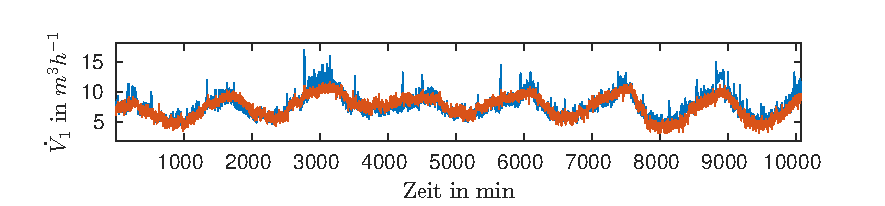
\includegraphics[width=0.8\textwidth]{val/v1.pdf}
     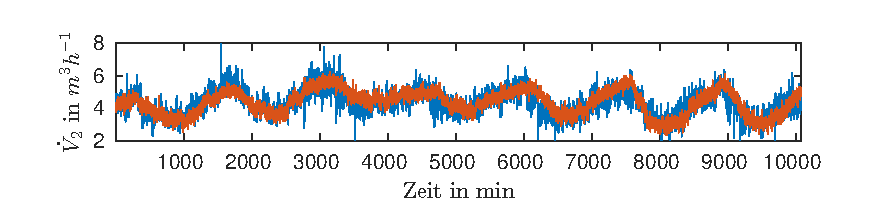
\includegraphics[width=0.8\textwidth]{val/v2.pdf}
     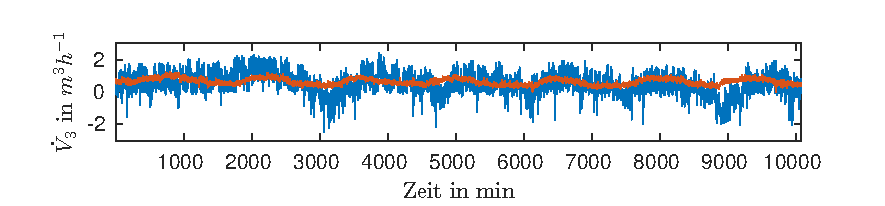
\includegraphics[width=0.8\textwidth]{val/v3.pdf}
     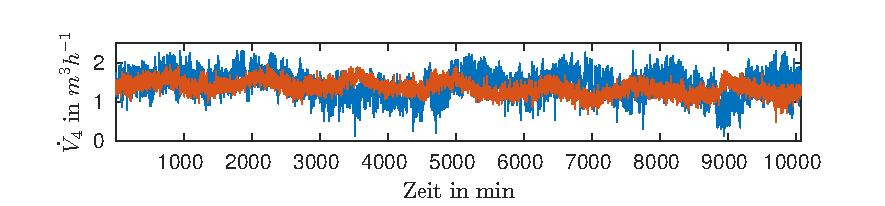
\includegraphics[width=0.8\textwidth]{val/v4.pdf}
     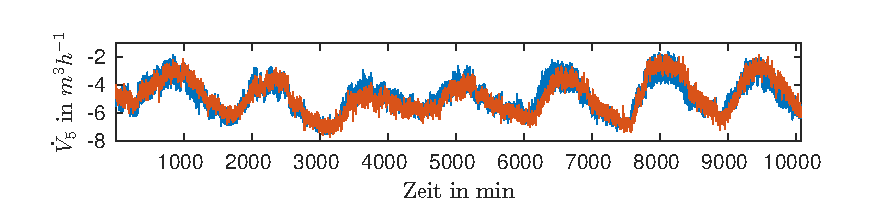
\includegraphics[width=0.8\textwidth]{val/v5.pdf}
  \caption{Ergebnis der Simulation von $\dot{V}_1 $ bis $\dot{V}_5$. Vergleich von Messdaten (\textcolor{blue}{blau}) und berechneten Werten (\textcolor{orange}{orange}).}
  \label{fig:v_val}
\end{figure}


\subsubsection{Vorlauftemperatur}\label{a:vorlauf_val}
Durchgehend gute Simulationsergebnisse werden f�r $T_{V,1}$ erzielt. Der Einfluss der Vorlauftemperatur der HZ1 ist f�r $T_{V,1}$ in allen untersuchten Betriebsmodi gro�, daher l�sst sich die Vorlauftemperatur in Punkt $P_1$ sehr gut allein durch durch $T_{V,HZ1}$ beschreiben wie Abbildung \ref{fig:v_val} zeigt.
\begin{figure}[htb] 
  \centering
     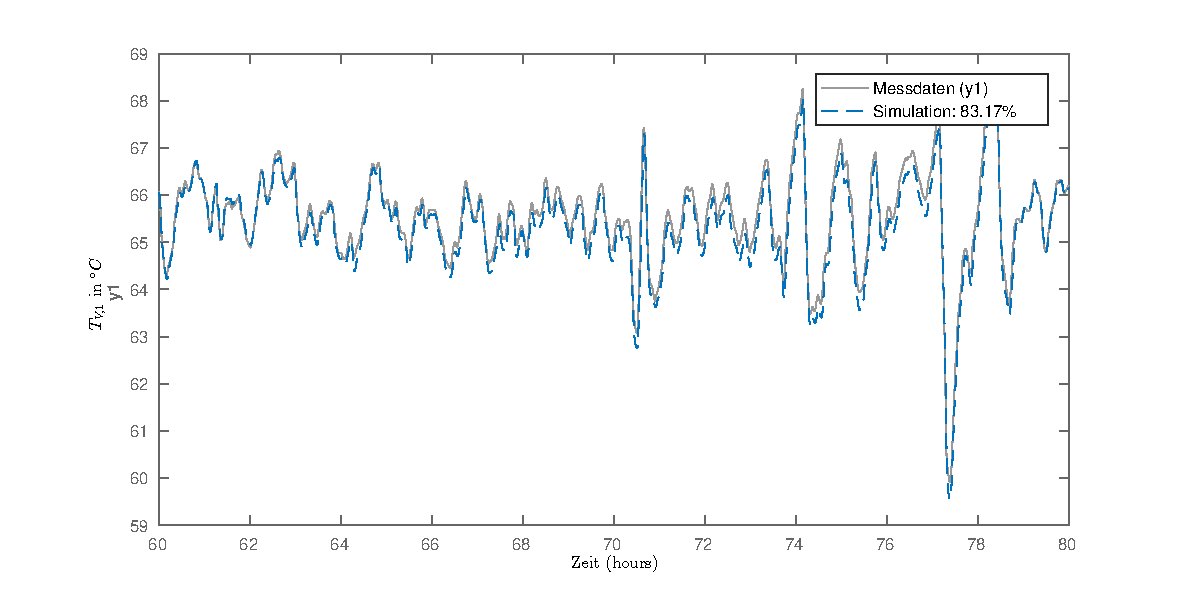
\includegraphics[width=1.0\textwidth]{val/tv1_zoom.pdf}
  \caption{Ausschnitt der Simulationsergebnisse zu $T_{V,1}$.}
  \label{fig:tv1_val}
\end{figure}
In Betriebsmodus 1 und 2 wird $T_{V,5}$ ebenfalls durch die Vorlauftemperatur der HZ1 beschrieben und zeigt �hnlich gute Ergebnisse. Sobald das System im Betriebsmodus 3 betrieben wird und eine Umkehr der Flie�richtung stattfindet, wird $T_{V,5}$  gem�� \ref{eq:tv_modell} durch $T_{V,4}$ berechnet. In Abbildung \ref{fig:tv5_modi} sind die Simulationsergebnisse f�r beide Flie�richtungen dargestellt. F�r den Betriebsmodus 3 erzielt die Simulation schlechtere  �bereinstimmungen, was auf eine ungen�gende Beschreibung allein durch $T_{V,4}$ hindeuten kann. Im untersuchten Zeitraum wurden nur wenige Flie�richtungswechsel am Punkt $P_{5}$ beobachtet, so dass eine genauere Analyse der Wechselwirkungen nicht weiterverfolgt werden konnte. \par
\begin{figure}[htb]
    \subfigure[$T_{V,5}$ im Betriebsmodus 1]{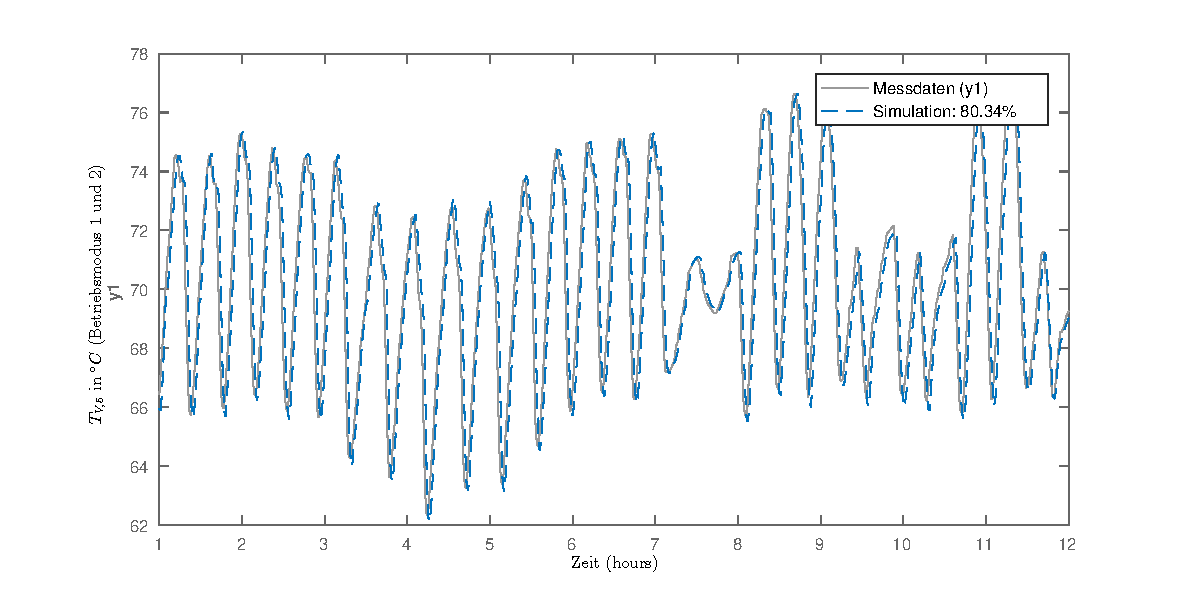
\includegraphics[width=0.49\textwidth]{val/tv5_zoom.pdf}}
    \subfigure[$T_{V,5}$ im Betriebsmodus 3]{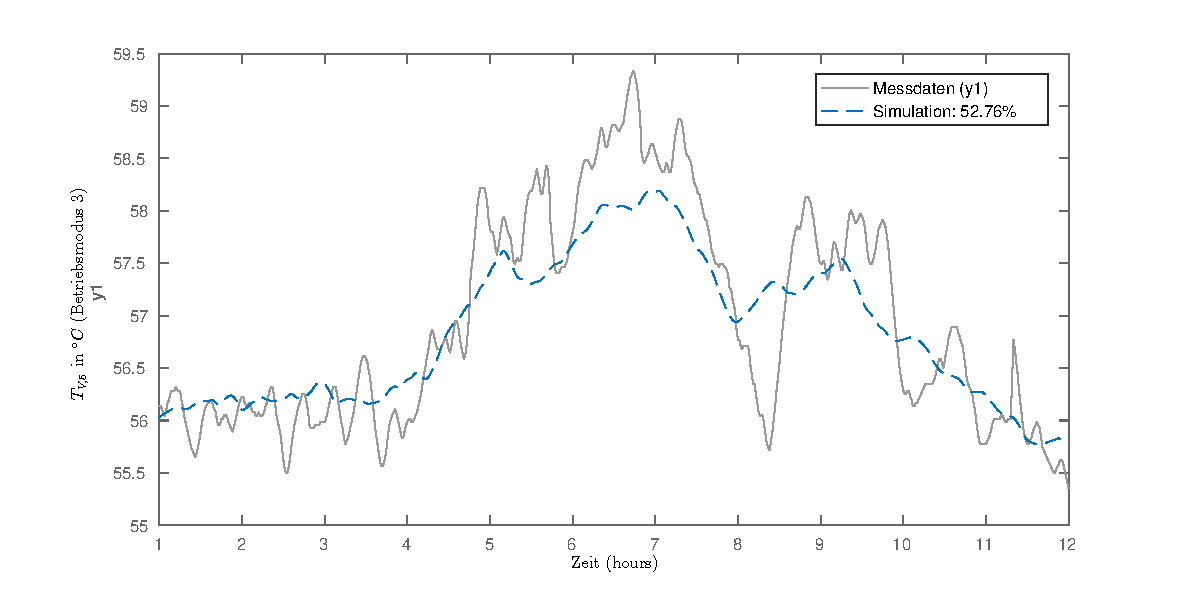
\includegraphics[width=0.49\textwidth]{val/tv5_b3.pdf}}
\caption{Vergleich der Vorhersageergebnisse f�r $T_{V,5}$ bei verschiedenen Flie�richtungen. Das Modell zeigt f�r negative Flie�richtung an $P_5$ bessere Ergebnisse (a) als f�r positive Flie�richtungen (b).}
\label{fig:tv5_modi}
\end{figure}
Vergleicht man die Simulationsergebnisse f�r $T_{V,2}$ mit den Messdaten, l�sst sich ein �hnlicher Signalverlauf erkennen, der aber zeitlich versetzt ist. Dies k�nnte darauf hindeuten, dass sich f�r $T_{V,2}$ bessere Simulationsergebnisse unter Ber�cksichtigung eines Totzeit�bertragungsgliedes erzielen lassen k�nnten. Dies k�nnte ein Ansatz f�r eine weiterf�hrende Optimierung des Modells sein.
\begin{figure}[htb] 
  \centering
     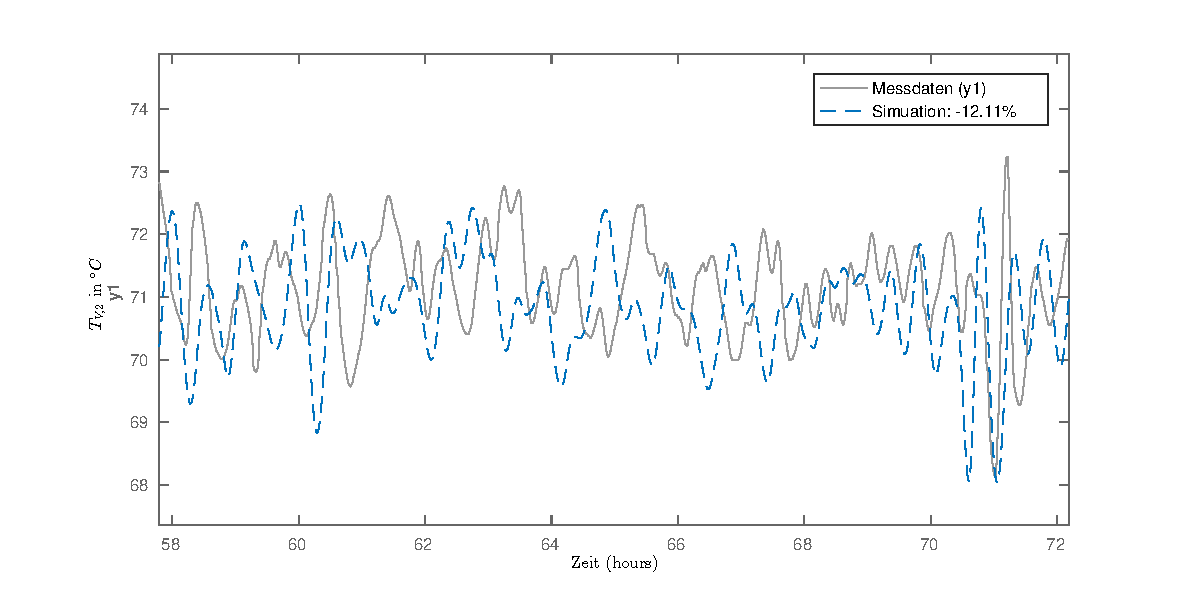
\includegraphics[width=1.0\textwidth]{val/tv2.pdf}
  \caption{Ausschnitt der Simulationsergebnisse zu $T_{V,2}$.}
  \label{fig:tv2_val}
\end{figure}
F�r $T_{V,3}$ lassen sich f�r die meisten Zeitr�ume nur schlechte Simulationsergebnisse erzielen, da ein h�ufiger Flie�richtungswechsel stattfindet, teilweise geschieht dies mehrmals am Tag. Da die Implementation des Modells in \textsc{Matlab} keine automatisierte Umstellung der Parameter bei einem Wechsel des Betriebsmodus vorsieht. Abbildung \ref{fig:tv3_modi} zeigt einen Vergleich der Simulationsergebisse f�r $T_{V,3}$ f�r den Zeitraum vom 16.04.2016 bis 23.04.2016, in dem h�ufige Flie�richtungswechsel stattfanden, mit den Simulationsergebnisse vom 07.07.2016 bis 17.07.2016, in dem die Anlage im Betriebsmodus 2 lief.\par
\begin{figure}[htb]
    \subfigure[$T_{V,3}$ bei h�ufigem Wechsel der Flie�richtung]{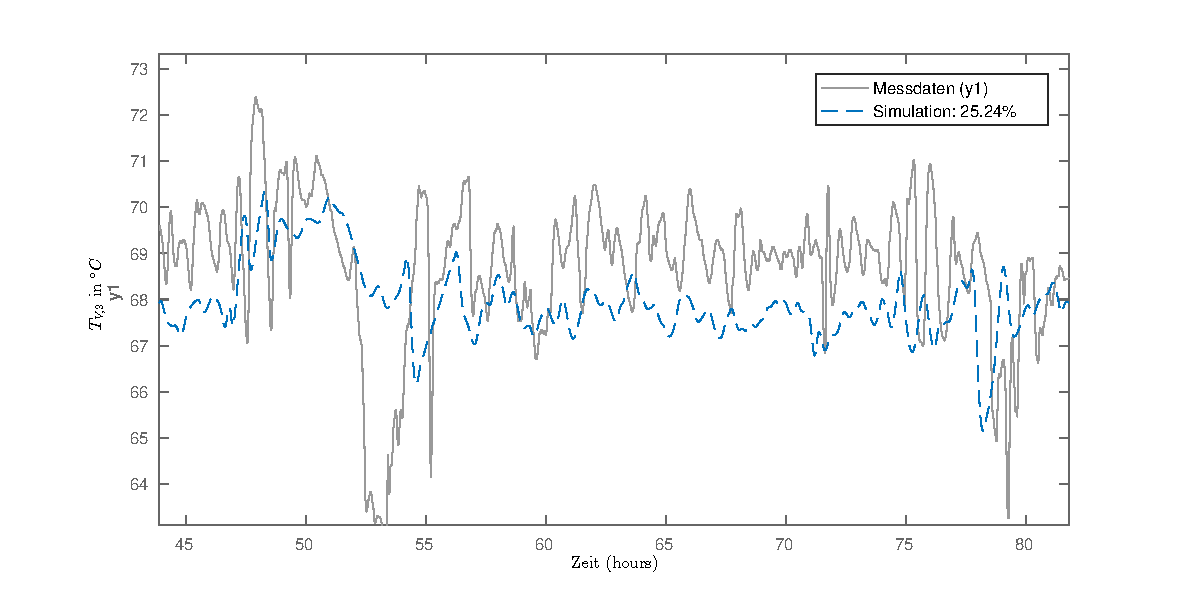
\includegraphics[width=0.49\textwidth]{val/tv3_schlecht.pdf}}
    \subfigure[$T_{V,5}$ bei konstanter Flie�richtung]{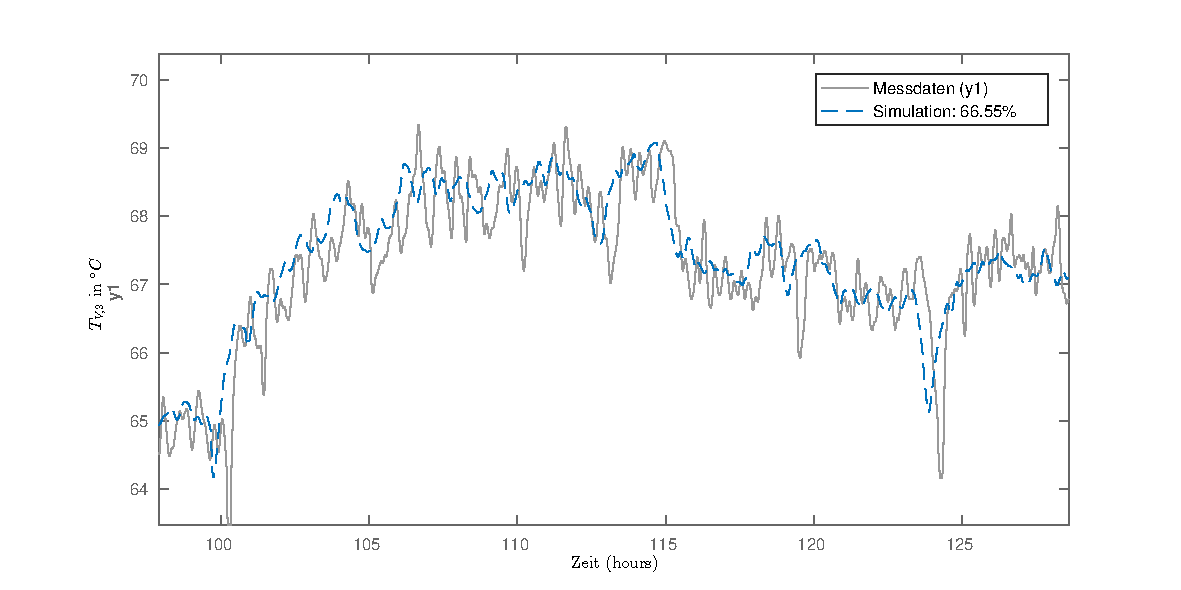
\includegraphics[width=0.49\textwidth]{val/tv3_gut.pdf}}
\caption{Vergleich der Vorhersageergebnisse f�r $T_{V,3}$ bei h�ufigen Flie�richtungswechseln (a) und bei konstanter Flie�richtung (b)}
\label{fig:tv3_modi}
\end{figure}
F�r $T_{V,4}$ werden durch das Modell durchgehend gute Vorhersageergebnisse mit NRMSE-Werten von rund 50 - 60 \% erzielt.

\subsubsection{W�rmeleistung}\label{a:waerme_val}
Da die W�rmeleistung mittels Black-box lediglich durch eine Abh�ngigkeit von der Au�entemperatur und der Vorlauftemperatur im selben Punkt abgesch�tzt wird, liefert die Simulation erwartungsgem�� vergleichsweise schlechte Vorhersageergebnisse. Auff�llig ist, dass f�r die Simulationen von $\dot{Q}_1$ , $\dot{Q}_2$ und $\dot{Q}_5$ insgesamt etwas bessere �bereinstimmungen zwischen Simulation und Messdaten erzielt werden k�nnen als f�r die Simulationen von $\dot{Q}_3$ und $\dot{Q}_4$ im selben Zeitraum, wie \ref{fig:q_gut} und \ref{fig:q_schlecht} zeigen.
\begin{figure}[htb]
  \centering
    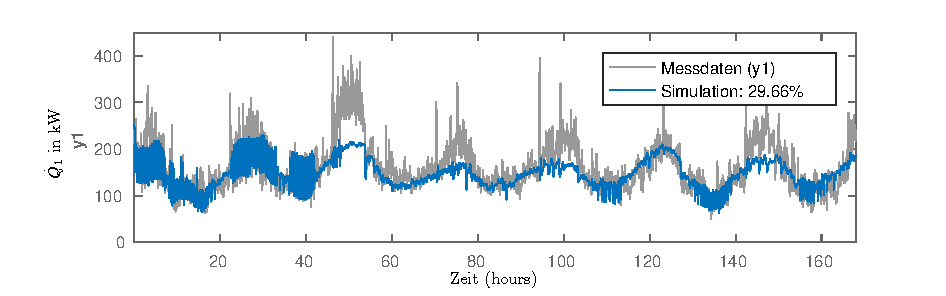
\includegraphics[width=0.8\textwidth]{val/q1.pdf}
    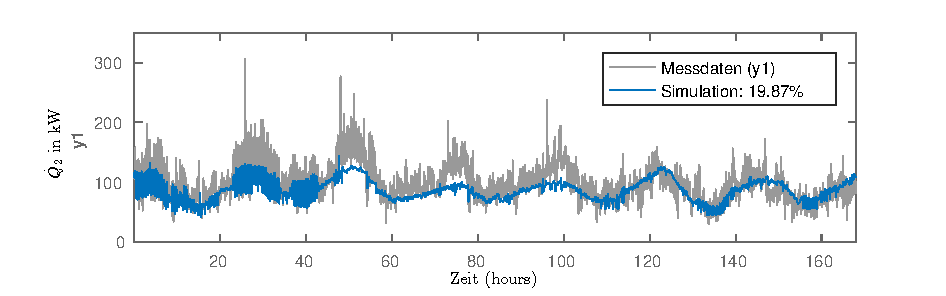
\includegraphics[width=0.8\textwidth]{val/q2.pdf}
    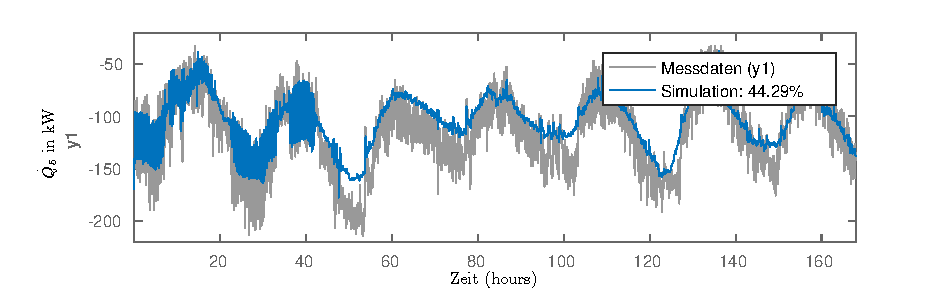
\includegraphics[width=0.8\textwidth]{val/q5.pdf}
\caption{Vergleich der Vorhersageergebnisse f�r $\dot{Q}_1$, $\dot{Q}_2$ und $\dot{Q}_5$. Der NRMSE liegt im Bereich von ca. 20 \% f�r alle drei Simulationen}
\label{fig:q_gut}
\end{figure}
F�r die W�rmeleistungen $\dot{Q}_3$ und $\dot{Q}_4$ werden insgesamt niedrigere Werte gemessen als f�r die anderen drei W�rmeleistungen, was vor allem auf die geringen Volumenstr�me in diesen Punkten zur�ckzuf�hren ist. Solch niedrige Volumenstr�me und die damit verbundenen niedrigen W�rmeleistungen k�nnten auf eine Unterversorgung der Verbraucher hindeuten, wobei der untersuchte Zeitraum f�r die Validierung am 11.04.2016 begann und damit bereits nicht mehr innerhalb der Heizperiode lag. Eine eventuelle Unterversorgung w�rde bei milden Au�entemperaturen nicht mehr so stark auffallen wie bei sehr niedrigen Au�entemperaturen. Sollte tats�chlich durch zu geringe Volumenstr�me weniger W�rmeleistung an den Punkten $P_3$ und $P_4$ abgenommen werden k�nnen, als tats�chlich von den Verbrauchern ben�tigt wird, sind auch die Simulationsergebnisse wenig aussagekr�ftig. Die W�rmeleistungsmodelle wurden anhand von Messdaten trainiert, ein fehlerhafter Betrieb der Anlage w�rde sich demnach auch in den Parametern des Modells widerspiegeln. Zur Verbesserung der Vorhersage und eventuell auch zur Fehlererkennung w�re eine Analyse des tats�chlichen Verbraucherverhaltens empfehlenswert.
\begin{figure}[htb]
  \centering
    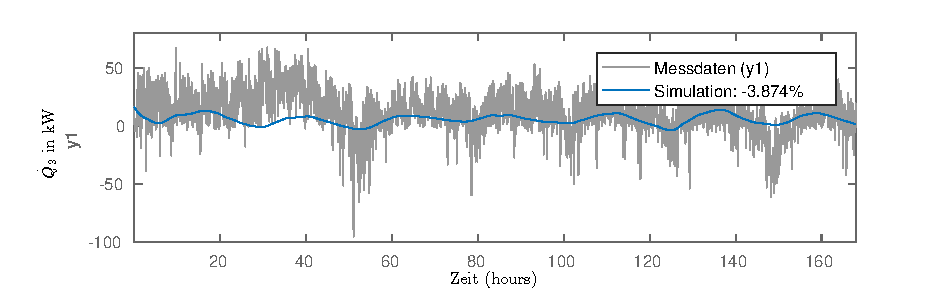
\includegraphics[width=0.8\textwidth]{val/q3.pdf}
    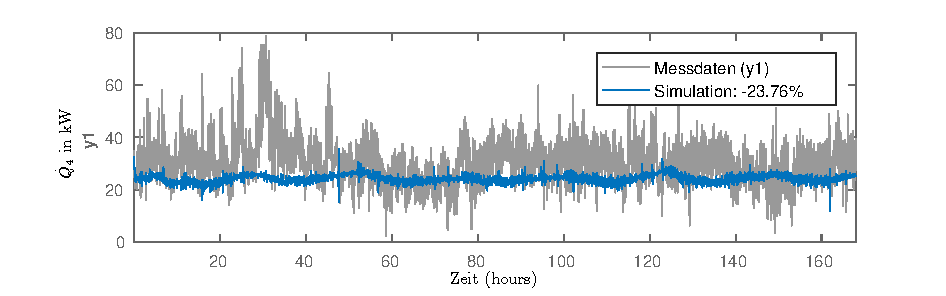
\includegraphics[width=0.8\textwidth]{val/q4.pdf}
\caption{Vergleich der Vorhersageergebnisse f�r $\dot{Q}_3$ und $\dot{Q}_4$. Der NRMSE liegt im Bereich f�r beide Simulationen im negativen Bereich weist deutlich schlechtere �bereinstimmung mit den Messdaten auf als die Simulationen f�r $\dot{Q}_1$, $\dot{Q}_2$ und $\dot{Q}_5$ }
\label{fig:q_schlecht}
\end{figure}

\subsection{Simulationsergebnisse des Gesamtmodells}
Das Gesamtmodell wurde evaluiert, indem die in Tabelle \ref{tab:input_output} beschriebenen Eingangs- und St�rgr��en dem Modell als Eingangssignale vorgegeben wurden. Die simulierten Ausgangssignale wurden aufgezeichnet und mit realen Messdaten verglichen, um die Qualit�t der Modellierung abzusch�tzen. Die Eingangssignale entsprechen Messdaten aus dem untersuchten Zeitraum vom 11. April 2016 bis 05. August 2016. Dabei wurde darauf geachtet, keine Messdaten zu nutzen, die ebenfalls zur Parameteridentifikation verwendet wurden. Die folgenden Kapitel beschreiben die Implementierung des Modell in \textsc{Matlab}, geben einen �berblick �ber die Valdierungsergebnisse und befassen sich mit eventuellen Fehlerquellen.

\subsubsection{Implementierung}
Das Modell wurde in der Entwicklungsumgebung \textsc{Matlab} inklusive der \textsc{System Identification Toolbox} implementiert. In einem Hauptskript kann der Anwender den Zeitraum festlegen, f�r den das Modell eine Vorhersage der Ausgangsgr��en berechnen soll. Dabei legt der Anwender das Startdatum sowie den Simulationszeitraum in Tagen, wobei eine Zeit von 7 Tagen voreingestellt ist. Das Skript erstellt anschlie�end die ben�tigten Datens�tze und f�hrt eine Parameteridentifikation �ber einen Zeitraum von 3 Tagen vor dem Startdatum durch. Die Systemmatrizen der Zustandsraummodelle und die Parameter des statischen Volumenstrommodells werden abgespeichert, um im darauffolgenden Simulationsschritt zur Verf�gung zu stehen. Die Simulationsergebnisse werden ebenfalls gespeichert und direkt im Anschluss an die Berechnung auf dem Bildschirm ausgegeben.

\subsubsection{Validierung}
Die Validierung der Teilmodelle erfolgte f�r jedes Teilsystem einzeln anhand realer Messdaten: die Messdaten wurden als Eingangssignal in jedes Teilsystem gegeben, das Systemverhalten wurde berechnet und die Ausgangssignale wurden mit Messdaten verglichen. F�r die Simulation des Gesamtmodells bestehen die Eingangssignale f�r einige Teilmodelle aus vorher simulierten Ausgangsgr��en anderer Teilmodelle, wie sich anhand des Blockschaltbildes erkennen l�sst. Liefert ein Teilmodell schlechte Simulationsergebnisse, wird dieser Fehler sich zwangsl�ufig fortpflanzen, weshalb insgesamt schlechtere Validierungsergebnisse f�r das Gesamtmodell erwartet werden k�nnen als f�r die Validierung der Teilmodelle. Tabelle \ref{tab:tv_sim_gesamt} zeigt die �bereinstimmung zwischen simulierten Vorlauftemperaturen und Messdaten bei verschiedenen Betriebsmodi. 
\begin{table}[b]
\centering
\caption{Vergleich der Simulationsergebnisse f�r $T_{V,1}$ bis $T_{V,5}$ f�r verschiedene Betriebsmodi}
\label{tab:tv_sim_gesamt}
\begin{tabular}{@{}llrrrrr@{}}
\toprule
                                 &              & \multicolumn{5}{c}{NRMSE in \%}   \\
                                 &              & $T_{V,1}$ & $T_{V,2}$ & $T_{V,3}$ & $T_{V,4}$ & $T_{V,5}$ \\ \midrule
\multirow{2}{*}{Betriebsmodus 1} & Gesamtmodell & 83.03   &  -14.32   & 12.46    &  52.53   &  80.34    \\
                                 & Teilmodell   & 83.03  &   -12.11  &  25.24   &   52.53   &  80.34    \\ 
\midrule
\multirow{2}{*}{Betriebsmodus 3} & Gesamtmodell & 78.58    &  -48.87   & 72.86   & 77.99   & 51.51     \\
                                 & Teilmodell   & 78.58    &  -39.45   & 72.79   & 77.99  &  62.96      \\ \bottomrule
\end{tabular}
\end{table}
Die �bereinstimmungen f�r die im Gesamtmodell berechneten Vorlauftemperaturen sind erwartungsgem�� etwas niedriger, wenn zur Berechnung die Temperatur des zuvor durchflossenen Punktes genutzt wird, wie das bei $T_{V,2}$ und $T_{V,3}$ in beiden Betriebsmodi sowie bei $T_{V,5}$ im Betriebsmodus 3 der Fall ist. Die schlechten �bereinstimmungswerte f�r $T_{V,2}$ im Betriebsmodus 3 resultieren aus einem Ausfall des Temperatursensons an dieser Stelle. Zu erkennen ist auch, dass f�r $T_{V,1}$ und $T_{V,4}$ sowie f�r $T_{V,5}$ im Betriebsmodus 1 gleiche �bereinstimmungen f�r das Gesamtmodell wie f�r die Teilmodelle erzielt werden. Diese Temperaturen werden nur durch die Vorlauftemperaturen der Erzeuger berechnet werden, nutzen also keine vorher anderweitig berechneten Eingangsgr��en. F�r Betriebsmodus 2 gab es im beobachteten Zeitraum keine Zeitspanne, in denen dieser Betriebsmodus ausreichend lange anhielt, um eine aussagekr�ftige Validierung durchzuf�hren.\par

\begin{table}[bt]
\centering
\caption{Vergleich der Simulationsergebnisse f�r $\dot{Q}_{1}$ bis $\dot{Q}_{2}$ f�r verschiedene Betriebsmodi}
\label{tab:q_sim_gesamt}
\begin{tabular}{@{}llrrrrr@{}}
\toprule
                                 &              & \multicolumn{5}{c}{NRMSE in \%}   \\
                                 &              &$\dot{Q}_{1}$&$\dot{Q}_{2}$&$\dot{Q}_{3}$ & $\dot{Q}_{4}$ &  $\dot{Q}_{5}$ \\ \midrule
\multirow{2}{*}{Betriebsmodus 1} & Gesamtmodell & 23.34   &  14.16   & -3.577   &  -8.638  &  42,88    \\
                                 & Teilmodell   & 23.34   &   15.86  &  -3.569  &  -8.858  &  42.88    \\ 
\midrule
\multirow{2}{*}{Betriebsmodus 3} & Gesamtmodell & 2.004   &  -16.57  &  1.433  & -1.627  & -4.336     \\
                                 & Teilmodell   & 3.722   &  12.81   &  1.226  & -1.301  &  -2.367      \\ \bottomrule
\end{tabular}
\end{table}


\subsubsection{Einfluss der Flussumkehr auf die Simulationsergebnisse}
\subsubsection{Fehlerquellen}

\section{Zusammenfassung und Ausblick}

%\section{Zusammenfassung und Ausblick}

Der vorliegenden Text gibt Studentinnen und Studenten, die am
Beginn der Niederschrift Ihrer Studien- oder Diplomarbeit am
Arbeitsbereich Regelungstechnik sind eine Anleitung, welche Punkte
zu beachten sind, damit diese Arbeit gelingt.


Sicherlich wurden nicht alle Aspekte des Schreibens aufgef�hrt.
F�r weitere Fragen steht Ihnen ja Ihr Betreuer ebenso zu
Verf�gung. Nutzen Sie den Dialog nach der Korrektur einzelner
Abschnitte als geeignetes Mittel zur Verbesserung Ihres
schriftlichen Textes!




 %% References ------------------------------------------
\bibliographystyle{ieeetr}
\bibliography{ba_lit}

 %%## Alternatively
%\cleardoublepage
%\begin{thebibliography}{99}
%\bibitem{Skelton97} R. Skelton, T. Iwasaki and K. Grigoriadis,
%"A unified approach to linear control design", Taylor \& Francis,
%London, UK, 1997
%\end{thebibliography}

 %% Appendix ---------------------------------------------
\appendix

\end{document}
